 \documentclass[aspectratio=169,xcolor=table]{beamer}
\usetheme{Madrid}\usecolortheme{seahorse}
\usepackage{booktabs,array}\usepackage{tikz}\usetikzlibrary{positioning,arrows.meta}
\usepackage{graphicx}
\graphicspath{{figures/}}
\setbeamertemplate{navigation symbols}{}
\setbeamertemplate{bibliography item}{}
\setbeamercolor{bibliography entry author}{fg=black}
\setbeamercolor{bibliography entry title}{fg=black}
\setbeamercolor{bibliography entry location}{fg=black}
\setbeamercolor{bibliography entry note}{fg=black}
\setbeamertemplate{footline}{\hfill\usebeamerfont{page number in head/foot}\usebeamercolor[fg]{page number in head/foot}\insertframenumber\,/\,\inserttotalframenumber\hspace{1.2em}\vspace{0.8em}}
\usepackage{tabularx}

\title[Compound Heat--Drought Stress]{Compound Heat--Drought Stress over India}
\subtitle{Are ecosystems hit harder when heat and drought strike together?\\[2pt] Mid-Evaluation, EVS Project \#19}
\author{Arnav Deshmukh \and Ayush Brajesh Roy \and Saksham Chitkara \and Gracy Garg \and Rudra Choudhary}
\institute{IIIT Hyderabad}
\date{October 9, 2026}

\begin{document}

\begin{frame}
  \titlepage
\end{frame}

% ---------- 1. Problem statement ----------
\begin{frame}{Problem statement}
    \begin{center}
        \Large \textbf{Compound Heat--Drought Stress: are ecosystems experiencing stronger combined impacts?}
        
        \vspace{1em}
        
        \large Does simultaneous heat and drought produce greater ecosystem stress than either disturbance alone?
        
        \vspace{1em}
        
        \normalsize Compare productivity and recovery during compound and single-stressor events.
    \end{center}
\end{frame}

% ---------- 2. Heat and drought rarely come alone ----------
\begin{frame}{Heat and drought rarely come alone}
\begin{columns}[c]
\column{0.54\textwidth}
\small
\begin{itemize}
  \item \textbf{Drought}: a shortage of water -- little rain, so the soil dries
    and roots cannot supply the plant.
  \item \textbf{Heatwave}: unusually high temperature. Hot air is
    ``thirstier'' (higher VPD) and pulls water out of leaves.
  \item \textbf{They feed each other:}
  \begin{itemize}
    \item dry soil has no water to evaporate, so the sun heats the air
      instead of cooling the land;
    \item heat speeds up evaporation, so the soil dries even faster.
  \end{itemize}
\end{itemize}
\column{0.44\textwidth}
\centering
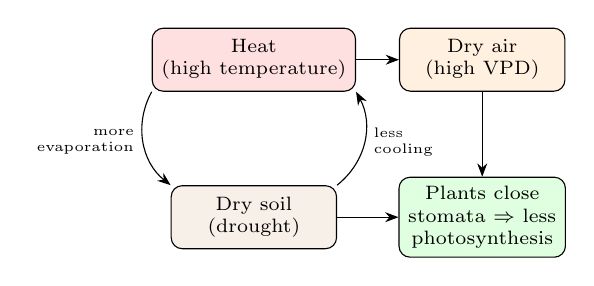
\begin{tikzpicture}[font=\scriptsize, >={Stealth},
  box/.style={draw, rounded corners, align=center, minimum width=2.1cm, minimum height=0.8cm}]
  \node[box, fill=red!12] (heat) at (0,0) {Heat\\(high temperature)};
  \node[box, fill=orange!12] (vpd) at (2.9,0) {Dry air\\(high VPD)};
  \node[box, fill=brown!12] (soil) at (0,-2) {Dry soil\\(drought)};
  \node[box, fill=green!12] (pl) at (2.9,-2) {Plants close\\stomata $\Rightarrow$ less\\photosynthesis};
  \draw[->] (heat) -- (vpd);
  \draw[->] (vpd) -- (pl);
  \draw[->] (soil) -- (pl);
  \draw[->] (heat.south west) to[bend right=40] node[left, align=right, font=\tiny]{more\\evaporation} (soil.north west);
  \draw[->] (soil.north east) to[bend right=40] node[right, align=left, font=\tiny]{less\\cooling} (heat.south east);
\end{tikzpicture}
\end{columns}
\end{frame}

% ---------- 3. How heat and drought affect plants ----------
\begin{frame}{How heat and drought affect plants?}
\small
\begin{itemize}
  \item Plants take up carbon by photosynthesis. The total amount is
    \textbf{gross primary productivity (GPP)} -- the base of food production.
  \item Leaves have tiny pores (\textbf{stomata}): CO$_2$ enters through them,
    and water escapes through the same pores.
  \item Under heat \emph{and} drought, plants are squeezed from both sides:
  \begin{itemize}
    \item \textbf{drought}: less water in the soil, so roots cannot supply the leaves;
    \item \textbf{heat}: the air demands more water, so stomata close
      $\Rightarrow$ less CO$_2$ uptake $\Rightarrow$ lower GPP;
    \item with no water to evaporate, leaves cannot cool themselves and overheat.
  \end{itemize}
   \item Past events:
  \begin{itemize}
    \item \textbf{Europe, summer 2003}: record heat with drought cut plant
      productivity by $\sim$30\%.
    \item \textbf{India, 2009}: the monsoon brought $\sim$22\% less rain than
      normal alongside above-normal temperatures; crops and natural
      vegetation browned across north and central India and the summer
      (kharif) harvest fell sharply.
  \end{itemize}
\end{itemize}
\end{frame}

% ---------- 4. Hypotheses ----------
\begin{frame}{Our hypotheses}
\renewcommand{\arraystretch}{1.4}
\begin{tabular}{@{}p{0.07\textwidth}>{\raggedright\arraybackslash}p{0.66\textwidth}p{0.2\textwidth}@{}}
\toprule
 & \textbf{Hypothesis} & \textbf{Status} \\
\midrule
H1 & GPP and NDVI are lower in compound months than in hot-only or dry-only months. & Tested \\
H2 & The compound effect is \emph{synergistic}: larger than heat effect + drought effect. & Tested \\
H3 & Recovery is slower after compound events than after droughts. & Final eval \\
H4 & The response differs by land cover and region (Peninsular vs North). & Final eval \\
\bottomrule
\end{tabular}

\end{frame}

% ---------- Workflow ----------
\begin{frame}{Workflow}
\centering
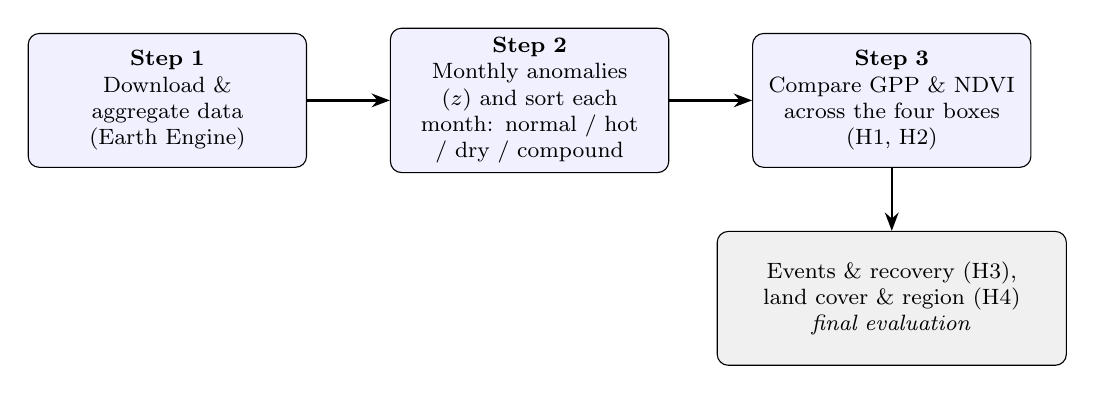
\begin{tikzpicture}[font=\footnotesize, >={Stealth},
  box/.style={draw, rounded corners, align=center, text width=3.3cm,
              minimum height=1.7cm, fill=blue!6},
  arr/.style={->, thick}]
  \node[box] (a) at (0,0) {\textbf{Step 1}\\Download \&\\aggregate data\\(Earth Engine)};
  \node[box] (b) at (4.6,0) {\textbf{Step 2}\\Monthly anomalies ($z$) and sort each month: normal / hot / dry / compound};
  \node[box] (c) at (9.2,0) {\textbf{Step 3}\\Compare GPP \& NDVI\\across the four boxes\\(H1, H2)};
  \node[box, fill=gray!12, text width=4.2cm, below=8mm of c] (d) {Events \& recovery (H3),\\land cover \& region (H4)\\\textit{final evaluation}};
  \draw[arr] (a) -- (b); \draw[arr] (b) -- (c); \draw[arr] (c) -- (d);
\end{tikzpicture}

\vspace{10pt}
\footnotesize Everything is scripted in Python (xarray, numpy, scipy) and checked by
automated tests. The analysis reruns from cached data in minutes.
\end{frame}

% ---------- 5. Data and metrics ----------
\begin{frame}{Data}
\small
All data put on one grid: boxes $\sim$27 km wide (0.25\textdegree), one value
per month, 4,481 boxes inside India.
\vspace{4pt}
\begin{itemize}
  \item \textbf{ERA5-Land} (1991--2024): reconstructed daily weather; its
    maximum temperature tells us which months are \emph{hot}.
  \item \textbf{SPEI} (1991--2024): a ready-made drought index; tells us
    which months are \emph{dry}.
  \item \textbf{CHIRPS} (1991--2024): rainfall from satellites and rain
    gauges; gives a second, rain-only drought check.
  \item \textbf{MODIS GPP} (2001--2022): satellite estimate of plant
    photosynthesis; our main measure of plant health.
  \item \textbf{MODIS NDVI} (2001--2022): satellite greenness; our second
    measure of plant health.
  \item \textbf{ESA WorldCover} (2021): land-cover map; tells us forest,
    cropland, shrubland or grassland, and removes non-vegetated areas.
\end{itemize}
\vspace{4pt}
% \footnotesize ERA5-Land also gives soil moisture and air dryness, used to
% explain \emph{why} plants are stressed.
\end{frame}


% (in Beamer, xcolor is already loaded, so pass the option instead: \documentclass[xcolor=table]{beamer})

\begin{frame}{Metrics at a glance}
\footnotesize
\renewcommand{\arraystretch}{1.25}
\begin{tabularx}{\textwidth}{@{} l X l @{}}
\rowcolor{orange!80}
\textbf{Metric} & \textbf{What it measures} & \textbf{How to read it} \\
\multicolumn{3}{@{}l}{\textit{\alert{Ecosystem response}}} \\
GPP & Carbon taken up by plants through photosynthesis (gC/m$^2$/month) & higher = more productive \\
NDVI & Canopy greenness from red and near-infrared reflectance (0--1) & higher = greener \\
\multicolumn{3}{@{}l}{\textit{\alert{Stress}}} \\
Tmax $z$ & Anomaly of the monthly mean daily maximum temperature & $\geq 1$: ``hot'' month \\
SPEI-3 & 3-month water balance: rain minus evaporative demand & $\leq -1$: ``dry'' month \\
SPI-3 & 3-month rainfall only (no temperature in it) & $\leq -1$: dry (robustness) \\
Soil moisture & Water in the top 1\,m of soil & lower = drier soil \\
VPD & Vapour-pressure deficit: how ``thirsty'' the air is & higher = more water stress \\
\multicolumn{3}{@{}l}{\textit{\alert{Statistics}}} \\
$z$-score & Distance from normal for that place and calendar month (in SDs) & 0 = normal; $-1$ = clearly low \\
Amplification & Compound effect $-$ (heat effect $+$ drought effect) & $<0$ synergy; $\approx 0$ additive \\
95\% CI & Year-block bootstrap: 1,000 resamples of whole years & excludes 0 = significant \\
\end{tabularx}
\end{frame}

% ---------- 6. Method: anomalies + four boxes ----------
\begin{frame}{Method: Four stress categories}
\begin{columns}[c]
\column{0.52\textwidth}
\small
\begin{itemize}
  \item \textbf{Why $z$-scores?} Raw values cannot be compared: May is
    always hotter than January, and deserts always have less GPP than
    forests.
  \item \textbf{Hot}: the month's average daily maximum temperature (Tmax $z) \ge 1$.
  \item \textbf{Dry}: SPEI-3 $\le -1$, meaning the last 3 months had clearly
    less water than usual (rain minus evaporative demand).
  \item Each of the 824,598 growing-season grid-months falls into one of
    four boxes: normal, hot-only, dry-only or compound.
  \item SPEI's demand term depends on temperature, so ``dry'' is partly
    driven by heat; we therefore repeat everything with SPI-3, which uses
    rainfall only.
\end{itemize}
\column{0.45\textwidth}
\centering\footnotesize
\begin{tabular}{c|c|c}
 & SPEI-3 $>-1$ & SPEI-3 $\le-1$ \\ \hline
Tmax $z<1$   & Normal   & Dry-only \\
             & 573,543  & 109,073 \\ \hline
Tmax $z\ge1$ & Hot-only & \textbf{Compound} \\
             & 79,717   & \textbf{62,265} \\
             &          & (7.6\%) \\
\end{tabular}

\vspace{6pt}
\scriptsize Number of growing-season grid-months in each box,\\
India, 2001--2022.
\end{columns}
\end{frame}
% ---------- Step 3 ----------
\begin{frame}{Step 3: how we test H1 and H2}
\begin{itemize}
  \item \textbf{H1}: average GPP $z$ (and NDVI $z$) in each box, and the differences between boxes.
  \item \textbf{H2}: compare the compound effect with the sum of the single effects. Each effect is measured relative to normal months:
  \[ \text{Amplification} = \Delta_{\text{compound}} - (\Delta_{\text{hot}} + \Delta_{\text{dry}}) \]
  \begin{itemize}
    \item $<0$: compound is worse than the sum $\Rightarrow$ \textbf{synergy};
    \item $\approx 0$: \textbf{additive};
    \item $>0$: less than the sum (\textbf{sub-additive}).
  \end{itemize}
  \item \textbf{Uncertainty}: 95\% confidence intervals from a \emph{year-block bootstrap}. We resample whole years (1,000 times), because neighbouring cells in the same year are not independent. A result is called significant when its interval excludes zero.
\end{itemize}
\end{frame}


% ---------- Where compound months happen ----------
\begin{frame}{Where compound months happen}
\begin{columns}[c]
\column{0.45\textwidth}
\centering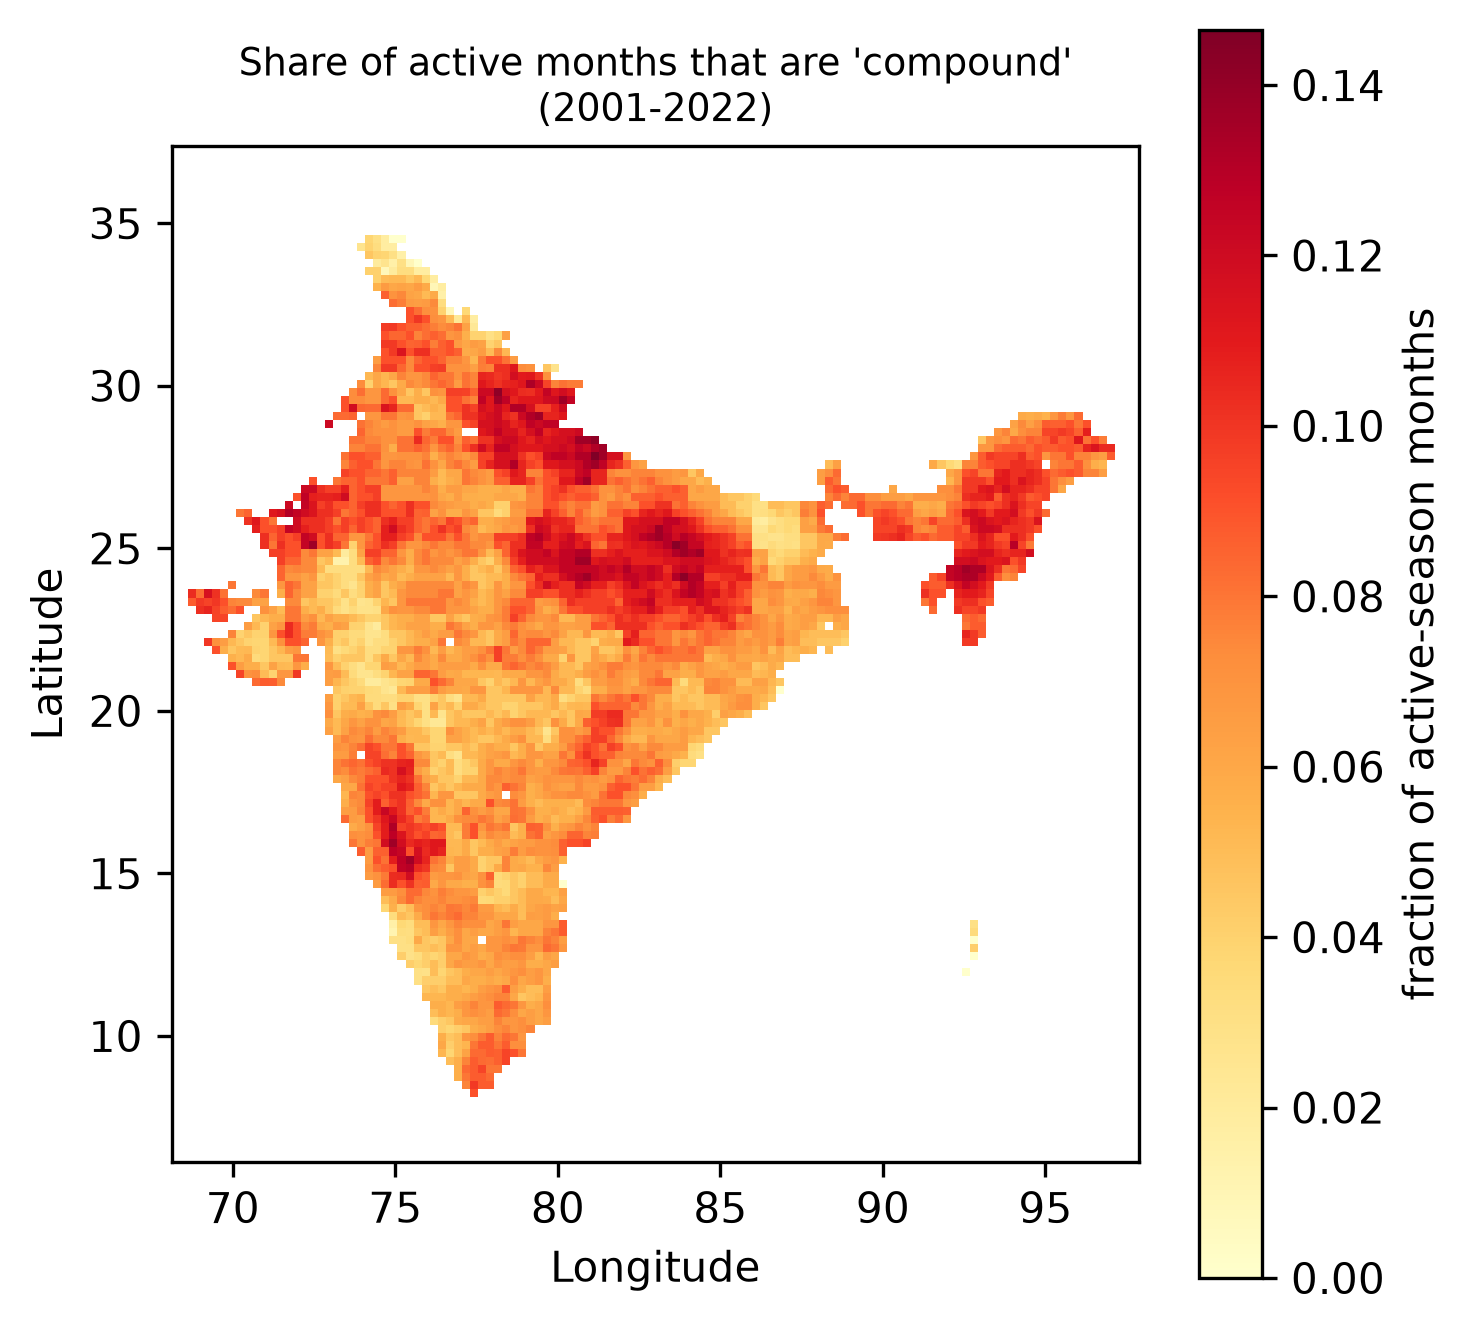
\includegraphics[width=\textwidth]{compound_share_map}
\column{0.5\textwidth}
\begin{itemize}
  \item Share of each cell's growing-season months that were compound, 2001--2022.
  \item Overall, 7.6\% of growing-season grid-months are compound.
  \item Hotspots: the northern plains, east-central India, the North-East, and a belt in the western Deccan (around 15--18°N).
  \item Both North and Peninsular India have more than 20,000 compound grid-months, enough for a reliable comparison.
\end{itemize}
\end{columns}
\end{frame}

% ---------- H1 figure ----------
\begin{frame}{H1: is vegetation hit harder in compound months?}
\centering
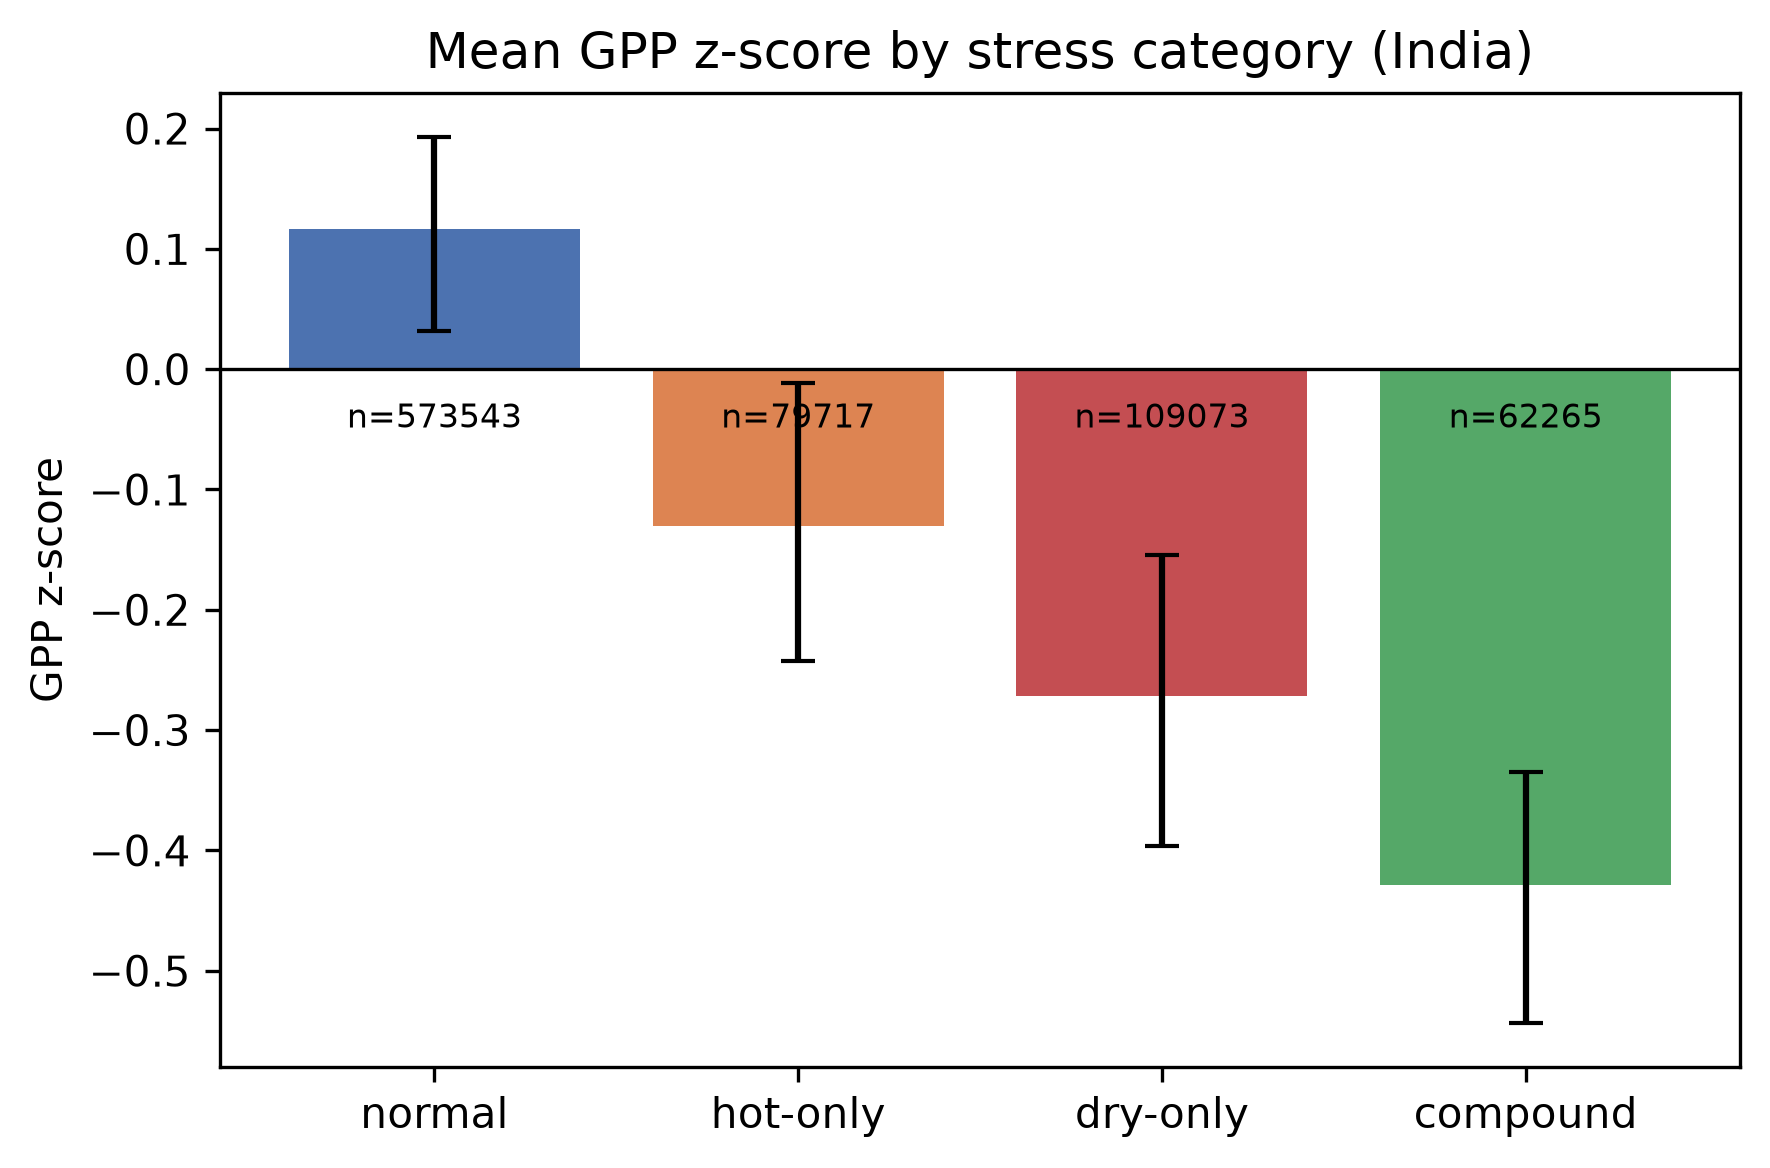
\includegraphics[width=0.46\textwidth]{h1_gpp_bars}\hfill
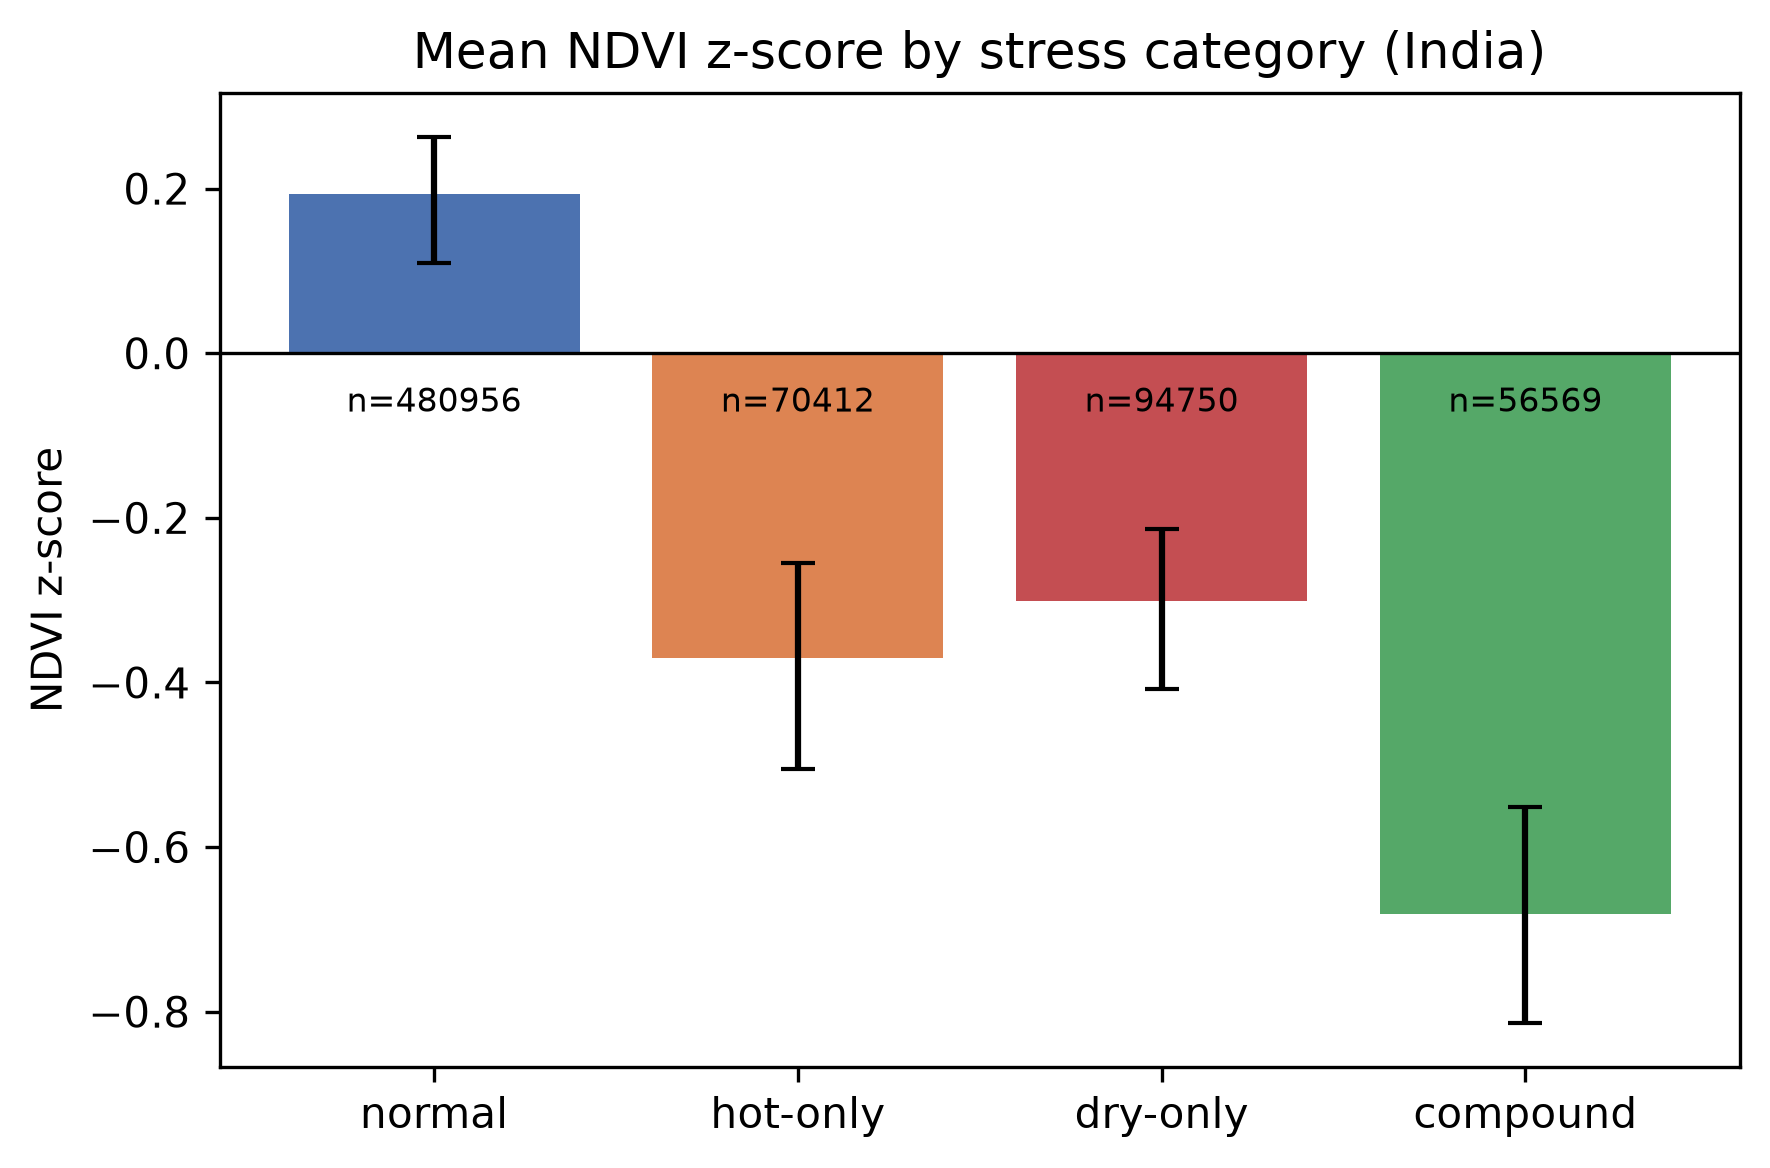
\includegraphics[width=0.46\textwidth]{h1_ndvi_bars}

\vspace{0.3em}
\footnotesize
\begin{tabular}{lcccc}
\toprule
Mean $z$ [95\% CI] & Normal & Hot-only & Dry-only & Compound \\
\midrule
GPP  & $+0.12$ & $-0.13$ [$-0.24, -0.01$] & $-0.27$ [$-0.40, -0.15$] & $-0.43$ [$-0.54, -0.33$] \\
NDVI & $+0.19$ & $-0.37$ [$-0.50, -0.26$] & $-0.30$ [$-0.41, -0.21$] & $-0.68$ [$-0.81, -0.55$] \\
\bottomrule
\end{tabular}
\end{frame}

% ---------- H1 result ----------
\begin{frame}{H1: result}
\small
\begin{itemize}
  \item All three stress types lower productivity and greenness significantly compared with normal months.
  \item \textbf{Compound months are the worst}, and significantly worse than either single stress:
  \begin{itemize}
    \item compound minus dry-only: GPP $-0.16$ [$-0.26, -0.04$], NDVI $-0.38$ [$-0.49, -0.28$];
    \item compound minus hot-only: GPP $-0.30$ [$-0.40, -0.21$], NDVI $-0.31$ [$-0.43, -0.21$].
  \end{itemize}
  \item Robust to the drought index. With rainfall-only SPI-3, compound minus dry-only is GPP $-0.26$ [$-0.37, -0.13$] and NDVI $-0.48$ [$-0.61, -0.35$].
  \item \textbf{Why?} Compound months combine the driest soils \emph{and} the thirstiest air:
\end{itemize}
\centering\footnotesize
\begin{tabular}{lcccc}
\toprule
 & Normal & Hot-only & Dry-only & Compound \\
\midrule
Root-zone soil moisture $z$ & $+0.29$ & $-0.75$ & $-0.38$ & $-1.04$ \\
Air dryness (VPD) $z$       & $-0.38$ & $+1.11$ & $+0.18$ & $+1.43$ \\
\bottomrule
\end{tabular}

\raggedright\small
\textbf{H1 supported.}
\end{frame}

% ---------- H2 figure ----------
\begin{frame}{H2: is the combination worse than the sum?}
\centering
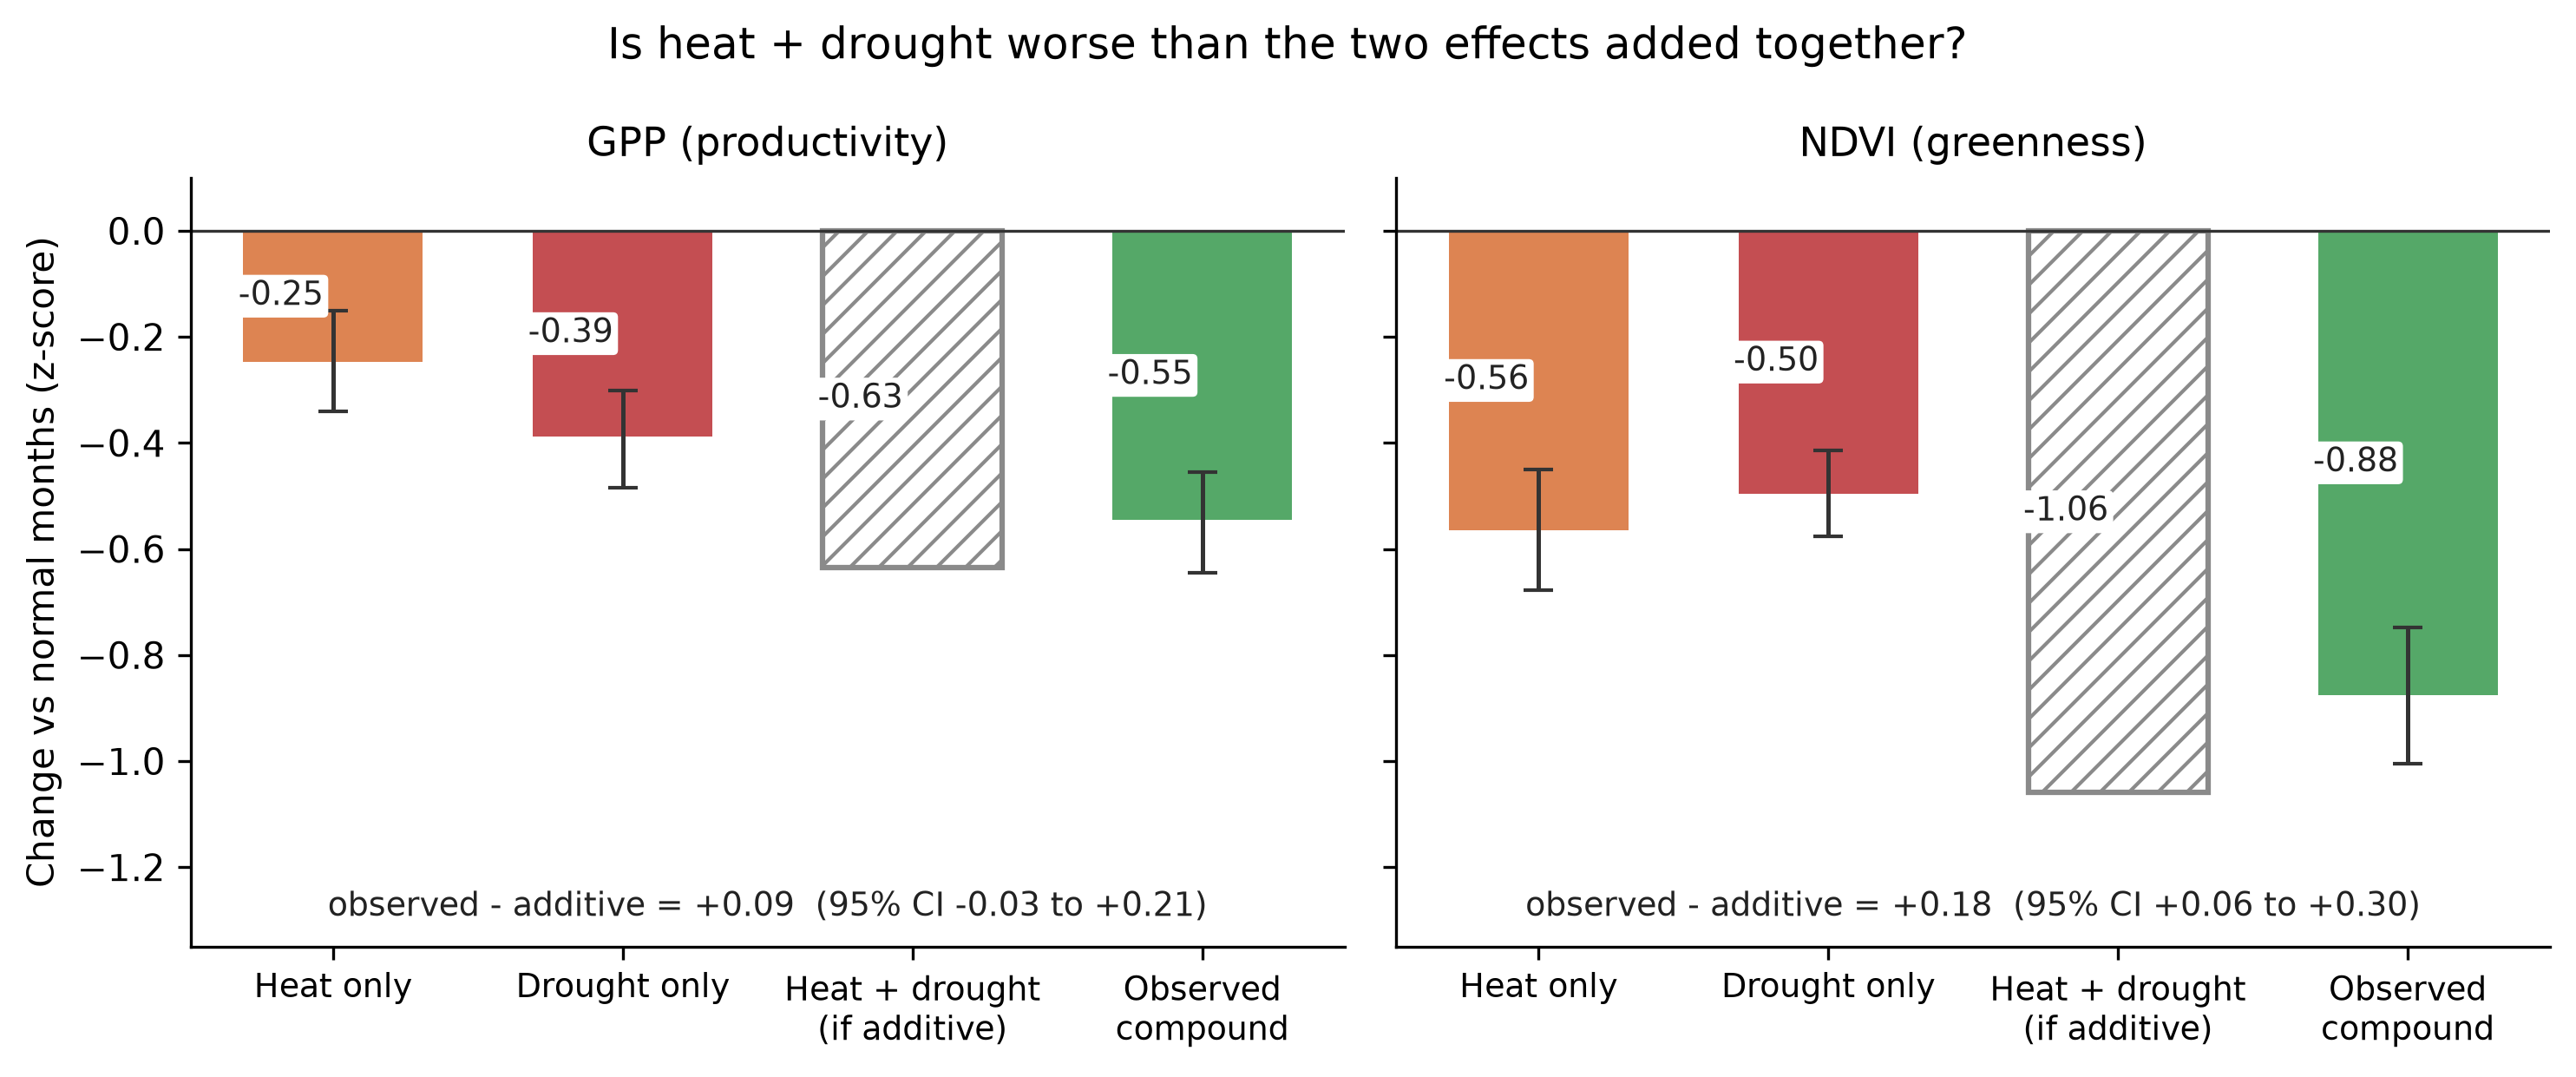
\includegraphics[width=0.88\textwidth]{h2_additivity}

\small Hatched bar: what we would expect if the two damages simply added up. Green bar: what actually happened in compound months.
\end{frame}

% ---------- H2 result ----------
\begin{frame}{H2: result}
\begin{columns}[c]
\column{0.48\textwidth}
Amplification $= \Delta_{\text{compound}} - (\Delta_{\text{hot}} + \Delta_{\text{dry}})$; $<0$ would mean synergy.

\vspace{0.6em}
\centering
\begin{tabular}{lrr}
\toprule
 & with SPEI-3 & with SPI-3 \\
\midrule
GPP  & $+0.09$ & $-0.00$ \\
     & {\scriptsize[$-0.03$, $+0.21$]} & {\scriptsize[$-0.12$, $+0.13$]} \\
NDVI & $+0.18$ & $+0.06$ \\
     & {\scriptsize[$+0.06$, $+0.30$]} & {\scriptsize[$-0.05$, $+0.18$]} \\
\bottomrule
\end{tabular}

\vspace{0.8em}
\raggedright
\textbf{H2 not supported} (for average productivity, India-wide).
\column{0.48\textwidth}
\begin{itemize}
  \item \textbf{No synergy}: the amplification is never significantly negative.
  \item Heat and drought damages roughly \textbf{add up}. Compound months are worse than either alone, but not worse than both together.
  \item With SPEI-3, NDVI is even slightly \emph{less} than additive, but this disappears with SPI-3. The drought definition matters.
\end{itemize}
\end{columns}
\end{frame}

% ---------- Response surface ----------
\begin{frame}{H2: Response Surface (A check without boxes)}
\begin{columns}[c]
\column{0.45\textwidth}
\centering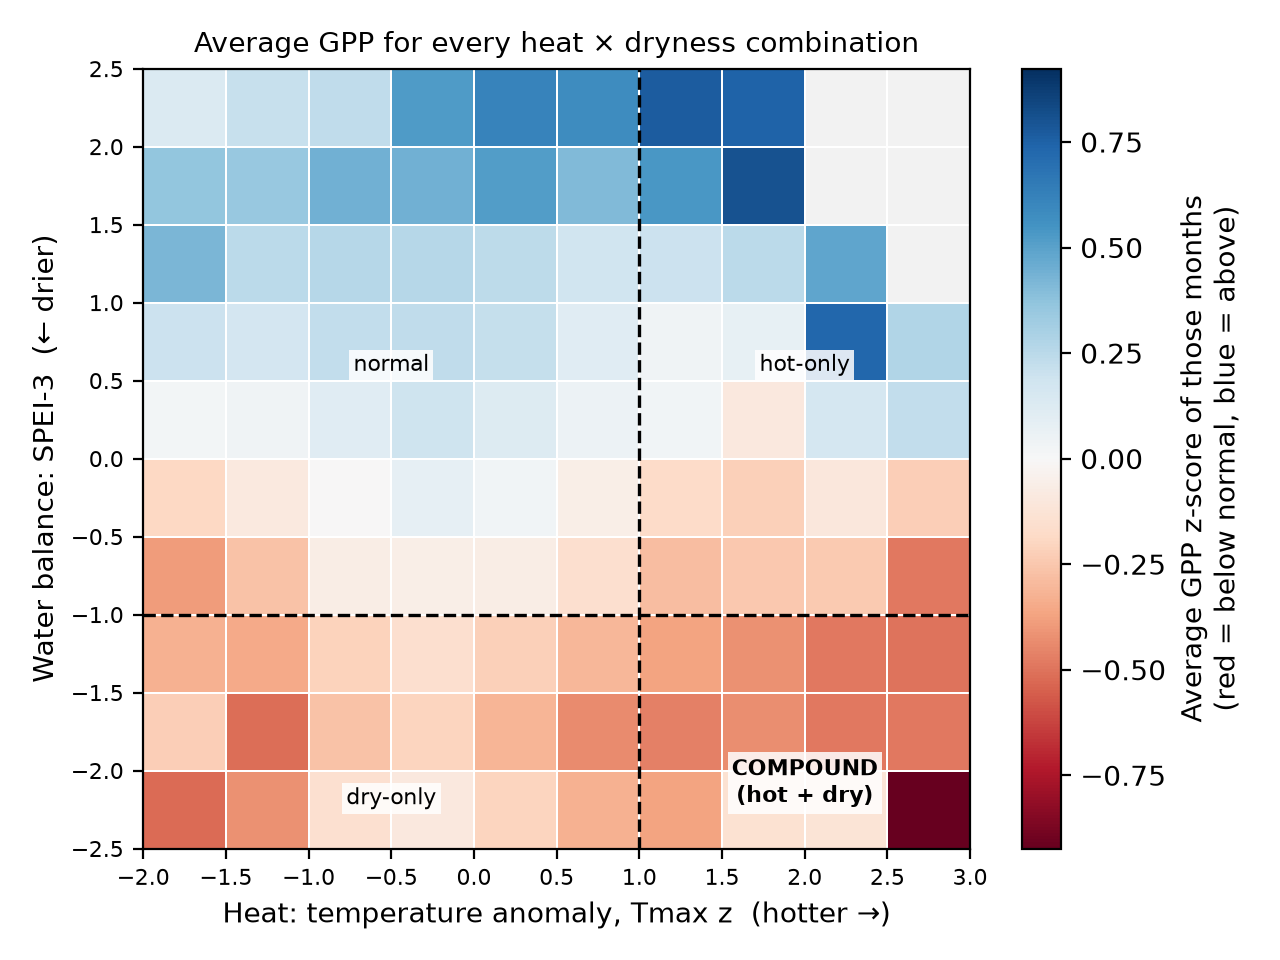
\includegraphics[width=\textwidth]{gpp_response_surface}
\column{0.53\textwidth}
\footnotesize
\textbf{What you are looking at}
\begin{itemize}
  \item $x$ = heat (Tmax $z$); $y$ = water balance (SPEI-3, lower = drier).
  \item Each square: average GPP $z$ of all grid-months in that range
    (red = below normal; grey = fewer than 30 grid-months).
  \item Dashed lines = our cut-offs; bottom-right = the compound box.
\end{itemize}
\vspace{4pt}
\textbf{What we see}
\begin{itemize}
  \item GPP falls as it gets drier: about $+0.5$ in the wettest rows,
    $-0.35$ in the driest.
  \item Worst square: hottest + driest corner ($-0.92$). Hot but wet months
    are not below normal.
  \item $\Rightarrow$ Dryness is the main driver and heat adds to it,
    consistent with additive effects.
\end{itemize}
\end{columns}
\end{frame}

% ---------- Observations ----------
\begin{frame}{Observations so far}
\small
\begin{itemize}
  \item \textbf{H1 supported.} Compound heat--drought months reduce productivity (GPP) and greenness (NDVI) significantly more than heat alone or drought alone. This holds for both drought indices.
  \item \textbf{H2 not supported.} The compound effect is about the \emph{sum} of the heat and drought effects, not more.
  \item \textbf{Mechanism.} Compound months have the driest soils and the thirstiest air at the same time.
  \item \textbf{Drought definition matters.} SPEI vs SPI changes the H2 details. Hot-only months also have dry soils (soil moisture $z=-0.75$), which rainfall-based indices miss.
  
\end{itemize}
\end{frame}

% ---------- Regression ----------
\begin{frame}{Improving H2: regression instead of four boxes}

\begin{block}{Why and what}
The four boxes use fixed cut-offs ($\pm1$) and ignore how strong each anomaly is.
So, by the final submission, we will move from four boxes to a
\alert{\textbf{regression fitted to every month's actual heat and dryness values}}.
\end{block}

\vspace{0.6em}
\[
\text{GPP} = a \times \text{heat} + b \times \text{dryness} + c \times (\text{heat} \times \text{dryness})
\]

\begin{itemize}
  \item $a$, $b$: how much GPP drops per unit of heat or dryness on its own
  \item $c < 0 \Rightarrow$ heat hurts more when it is also dry (synergy)
  \item One direct test with a confidence interval, and no arbitrary cut-offs
\end{itemize}

\end{frame}



\begin{frame}{Further work}

\begin{columns}[T]
  \begin{column}{0.32\textwidth}
    \textbf{\alert{H3: Recovery}}
    \begin{itemize}
      \item Time for vegetation to recover after each event
      \item Compound vs drought-only at the same drought severity
    \end{itemize}
  \end{column}

  \begin{column}{0.32\textwidth}
    \textbf{\alert{H4: Land cover \& region}}
    \begin{itemize}
      \item Forests, croplands, grasslands
      \item Peninsular vs North India
    \end{itemize}
  \end{column}

  \begin{column}{0.32\textwidth}
    \textbf{\alert{Beyond India}}
    \begin{itemize}
      \item Repeat the analysis for another country
      \item Does India's ``additive'' result hold elsewhere?
    \end{itemize}
  \end{column}
\end{columns}

\vfill
{\small All our datasets cover the globe (CHIRPS: 50\textdegree S--50\textdegree N), so the same pipeline can be pointed at a new region.}

\end{frame}

\end{document}